



%%%%%%%%%%%%%%%%%%%%%%%%%%%%%%%%%%%%%%%%%
% Beamer Presentation
% LaTeX Template
% Version 1.0 (10/11/12)
%
% This template has been downloaded from:
% http://www.LaTeXTemplates.com
%
% License:
% CC BY-NC-SA 3.0 (http://creativecommons.org/licenses/by-nc-sa/3.0/)
%
%%%%%%%%%%%%%%%%%%%%%%%%%%%%%%%%%%%%%%%%%

%----------------------------------------------------------------------------------------
%	PACKAGES AND THEMES
%----------------------------------------------------------------------------------------

\documentclass[aspectratio=169]{beamer}

\mode<presentation> {


% The Beamer class comes with a number of default slide themes
% which change the colors and layouts of slides. Below this is a list
% of all the themes, uncomment each in turn to see what they look like.

%\usetheme{default}
%\usetheme{AnnArbor}
%\usetheme{Antibes}
%\usetheme{Bergen}
%\usetheme{Berkeley}
%\usetheme{Berlin}
%\usetheme{Boadilla}
%\usetheme{CambridgeUS}
%\usetheme{Copenhagen}
%\usetheme{Darmstadt}
%\usetheme{Dresden}
%\usetheme{Frankfurt}
%\usetheme{Goettingen}
%\usetheme{Hannover}
%\usetheme{Ilmenau}
%\usetheme{JuanLesPins}
%\usetheme{Luebeck}
\usetheme{Madrid}
%\usetheme{Malmoe}
%\usetheme{Marburg}
%\usetheme{Montpellier}
%\usetheme{PaloAlto}
%\usetheme{Pittsburgh}
%\usetheme{Rochester}
%\usetheme{Singapore}
%\usetheme{Szeged}
%\usetheme{Warsaw}

% As well as themes, the Beamer class has a number of color themes
% for any slide theme. Uncomment each of these in turn to see how it
% changes the colors of your current slide theme.

%\usecolortheme{albatross}
%\usecolortheme{beaver}
%\usecolortheme{beetle}
%\usecolortheme{crane}
%\usecolortheme{dolphin}
%\usecolortheme{dove}
%\usecolortheme{fly}
%\usecolortheme{lily}
%\usecolortheme{orchid}
%\usecolortheme{rose}
%\usecolortheme{seagull}
%\usecolortheme{seahorse}
%\usecolortheme{whale}
%\usecolortheme{wolverine}

%\setbeamertemplate{footline} % To remove the footer line in all slides uncomment this line
%\setbeamertemplate{footline}[page number] % To replace the footer line in all slides with a simple slide count uncomment this line
\usepackage{amsmath}
\usepackage{selinput}   
\usepackage[boxed]{algorithm}
\usepackage{algorithmic}   % Halbautomatische Auswahl der Eingabecodierung
\SelectInputMappings{      % mit Hilfe ausgewählter Glyphen
  adieresis={ä},	   % siehe: http://partners.adobe.com/public/developer/en/opentype/glyphlist.txt
  germandbls={ß},
  Euro={€}
}

\definecolor{UOSred}{rgb}{0.6745098039215686, 0.02352941176470588, 0.2039215686274510} % UBC Blue (primary)
\definecolor{UOSgrey}{rgb}{0.8117647058823529, 0.8117647058823529, 0.8117647058823529} % UBC Grey (secondary)

\setbeamercolor{palette primary}{bg=UOSred,fg=white}
\setbeamercolor{palette secondary}{bg=UOSred,fg=white}
\setbeamercolor{palette tertiary}{bg=UOSred,fg=white}
\setbeamercolor{palette quaternary}{bg=UOSred,fg=white}
\setbeamercolor{structure}{fg=UOSred} % itemize, enumerate, etc
\setbeamercolor{section in toc}{fg=UOSred} % TOC sections

%gets rid of bottom navigation bars
\setbeamertemplate{footline}[frame number]{}

%gets rid of bottom navigation symbols
\setbeamertemplate{navigation symbols}{}

\addtobeamertemplate{footline}{%
  \leavevmode%
  \hbox{%
  \begin{beamercolorbox}[wd=\paperwidth,ht=2.25ex,dp=1ex,center]{author in head/foot}%
     \insertsectionnavigationhorizontal{\paperwidth}{}{}
  \end{beamercolorbox}}%

}

% Override palette coloring with secondary
\setbeamercolor{subsection in head/foot}{bg=UOSgrey,fg=white}

%\setbeamertemplate{navigation symbols}{} % To remove the navigation symbols from the bottom of all slides uncomment this line
}
\usepackage{hyperref}
\usepackage{graphicx} % Allows including images
\usepackage{grffile}
\usepackage{booktabs} % Allows the use of \toprule, \midrule and \bottomrule in tables
\graphicspath{{images/}}
%----------------------------------------------------------------------------------------
%	TITLE PAGE
%----------------------------------------------------------------------------------------

\title[Phase 2]{Übungsprojekt Phase 3} % The short title appears at the bottom of every slide, the full title is only on the title page

\author{T. Adam, M. ben Ahmed} % Your name
\institute[UOS] % Your institution as it will appear on the bottom of every slide, may be shorthand to save space
{

Universität Osnabrück \\ % Your institution for the title page

\medskip
\textit{Æ} % Your email address


}
\date{\today} % Date, can be changed to a custom date

\begin{document}

\begin{frame}
\titlepage % Print the title page as the first slide
\end{frame}


%----------------------------------------------------------------------------------------
%	PRESENTATION SLIDES
%----------------------------------------------------------------------------------------



\begin{frame}
\frametitle{Phase 2 - Heuristiken für das Point Labeling Problem}
\begin{columns}[c] % The "c" option specifies centered vertical alignment while the "t" option is used for top vertical alignment
	
	\column{.30\textwidth} % Left column and width
	\textbf{Greedy}
	\begin{itemize}
		\item trivialer Algorithmus
		\item setze Label nach fester Reihenfolge
		\item wenn das nicht funktioniert $\rightarrow$ \texttt{continue}
		\item []
		
		
	\end{itemize}
	
	\column{.30\textwidth} % Right column and width
	\textbf{Normals}
	\begin{itemize}
		\item geometrisch
		\item bestimmt Zentrum der Nachbarschaft
		\item startet mit 'dichten' Punkten
		\item []
		\item []
		
	\end{itemize}
	

	\column{.30\textwidth} % Right column and width
	\textbf{Simulated Annealing}
	\begin{itemize}
		\item Metaheuristik
		\item benötigt Startlösung
		\item betrachtet zufällige Nachbarschaften
		\item variiert Verschlechterungstoleranz
		\item []
	\end{itemize}

\end{columns}
\end{frame}

%------------------------------------------------

\begin{frame}
	\frametitle{Phase 2 - Heuristiken}
	\begin{columns}[c] % The "c" option specifies centered vertical alignment while the "t" option is used for top vertical alignment
		
		\column{.45\textwidth} % Left column and width
		\textbf{Normals:}
		\begin{itemize}
			\item Geometrischer Ansatz
		\end{itemize}
		
		\column{.45\textwidth} % Right column and width
		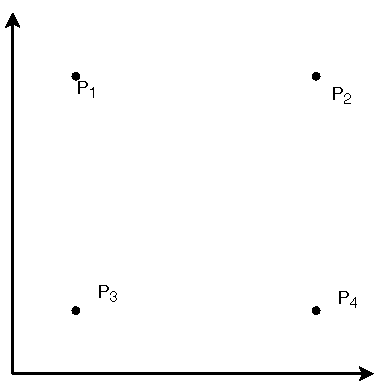
\includegraphics[scale=.7]{normals_scheme.pdf}
		
		
		
	\end{columns}
	\end{frame}
	
%------------------------------------------------


\begin{frame}
	\frametitle{Phase 2 - Heuristiken}
	\begin{columns}[c] % The "c" option specifies centered vertical alignment while the "t" option is used for top vertical alignment
		
		\column{.45\textwidth} % Left column and width
		\textbf{Normals:}
		\begin{itemize}
			\item Geometrischer Ansatz
			\item Berechnet Zentrum der Nachbarschaft
			
		\end{itemize}
		
		\column{.45\textwidth} % Right column and width
		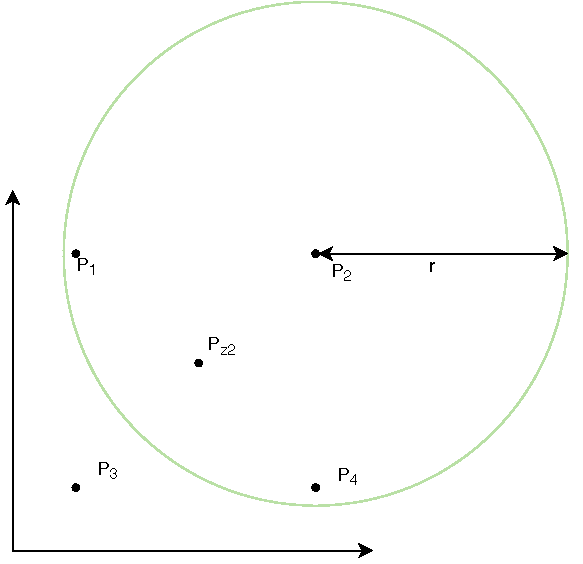
\includegraphics[scale=.7]{normals_centroid.pdf}
		
		
		
	\end{columns}
	\end{frame}
	
%------------------------------------------------


\begin{frame}
	\frametitle{Phase 2 - Heuristiken}
	\begin{columns}[c] % The "c" option specifies centered vertical alignment while the "t" option is used for top vertical alignment
		
		\column{.45\textwidth} % Left column and width
		\textbf{Normals:}
		\begin{itemize}
			\item Geometrischer Ansatz
			\item Berechnet Zentrum der Nachbarschaft
			\item Weist Punkten Normalen zu
			
		\end{itemize}
		
		\column{.45\textwidth} % Right column and width
		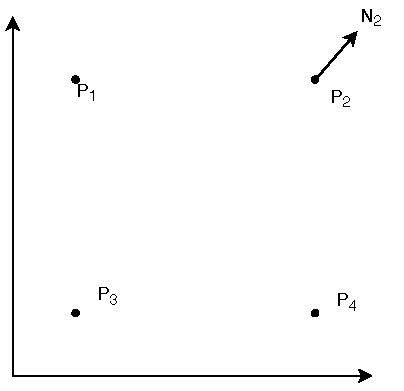
\includegraphics[scale=.7]{normals_normal.pdf}
		
		
		
	\end{columns}
	\end{frame}
	
%------------------------------------------------


\begin{frame}
	\frametitle{Phase 2 - Heuristiken}
	\begin{columns}[c] % The "c" option specifies centered vertical alignment while the "t" option is used for top vertical alignment
		
		\column{.45\textwidth} % Left column and width
		\textbf{Normals:}
		\begin{itemize}
			\item Geometrischer Ansatz
			\item Berechnet Zentrum der Nachbarschaft
			\item Weist Punkten Normalen zu
			\item Label wird in Richtung der Normale gesetzt
			
		\end{itemize}
		
		\column{.45\textwidth} % Right column and width
		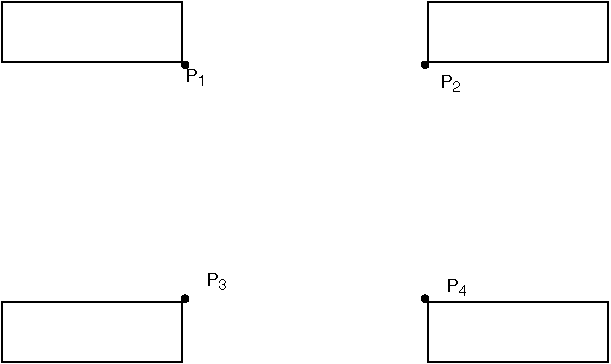
\includegraphics[scale=.6]{normal_finished.pdf}
		
		
		
	\end{columns}
	\end{frame}
	
%------------------------------------------------


\begin{frame}
	\frametitle{Phase 2 - Heuristiken}
	\begin{columns}[c] % The "c" option specifies centered vertical alignment while the "t" option is used for top vertical alignment
		
		\column{.45\textwidth} % Left column and width
		\textbf{Idee:}
		\begin{itemize}
			\item  Vermeidet Konflikte indem Ballungszentren gemieden werden
			\item Platziere Punkte mit dichter Nachbarschaft zuerst
		\end{itemize}
		\column{.45\textwidth} % Right column and width
		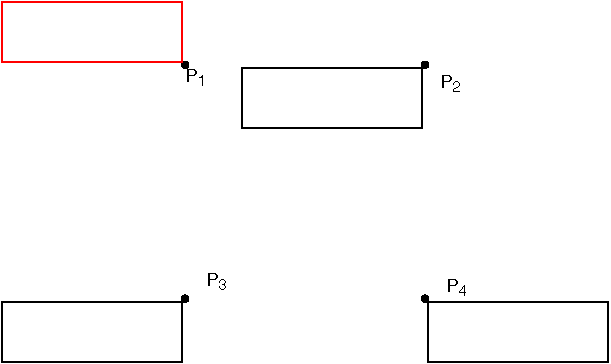
\includegraphics[scale=.6]{normals_conflict.pdf}
		
		
		
	\end{columns}
	\end{frame}
	
%------------------------------------------------



\begin{frame}
	\frametitle{Phase 2 - Heuristiken}
	\begin{columns}[c] % The "c" option specifies centered vertical alignment while the "t" option is used for top vertical alignment
		
		\column{.45\textwidth} % Left column and width
		\textbf{Simulated Annealing:}
		\begin{itemize}
			\item Es werden Nachbarschaften von Lösungen  betrachtet
			\item Label Position zufällig ändern und neue Lösung auswerten
		\end{itemize}
		\column{.45\textwidth} % Right column and width
		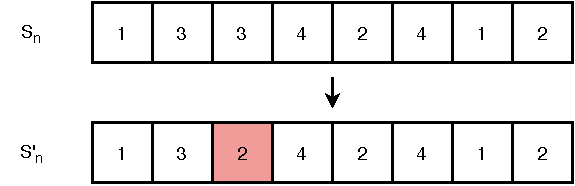
\includegraphics[scale=.6]{sa_representation.pdf}
		
		
		
	\end{columns}
	\end{frame}
	
%------------------------------------------------



\begin{frame}
	\frametitle{Phase 2 - Heuristiken}
	\begin{columns}[c] % The "c" option specifies centered vertical alignment while the "t" option is used for top vertical alignment
		
		\column{.55\textwidth} % Left column and width
		\textbf{Simulated Annealing:}
		\begin{itemize}
			\item Bessere und gleiche Lösungen werden immer akzeptiert
			\item Verschlechterungen werden mit bestimmter Wahrscheinlichkeit akzeptiert
		\end{itemize}
		\column{.45\textwidth} % Right column and width
		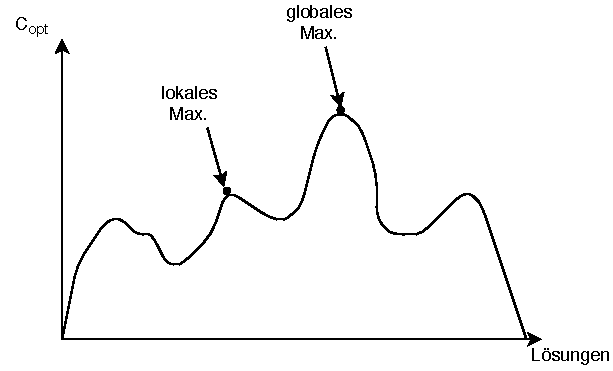
\includegraphics[scale=.6]{sa_maximum.pdf}
		
		
		
	\end{columns}
	\end{frame}
	
%------------------------------------------------
\begin{frame}
	\frametitle{Phase 2 - Instanzen}
	\textbf{Cluster}
	\begin{columns}[c] % The "c" option specifies centered vertical alignment while the "t" option is used for top vertical alignment
		
		\column{.9\textwidth} % Left column and width
		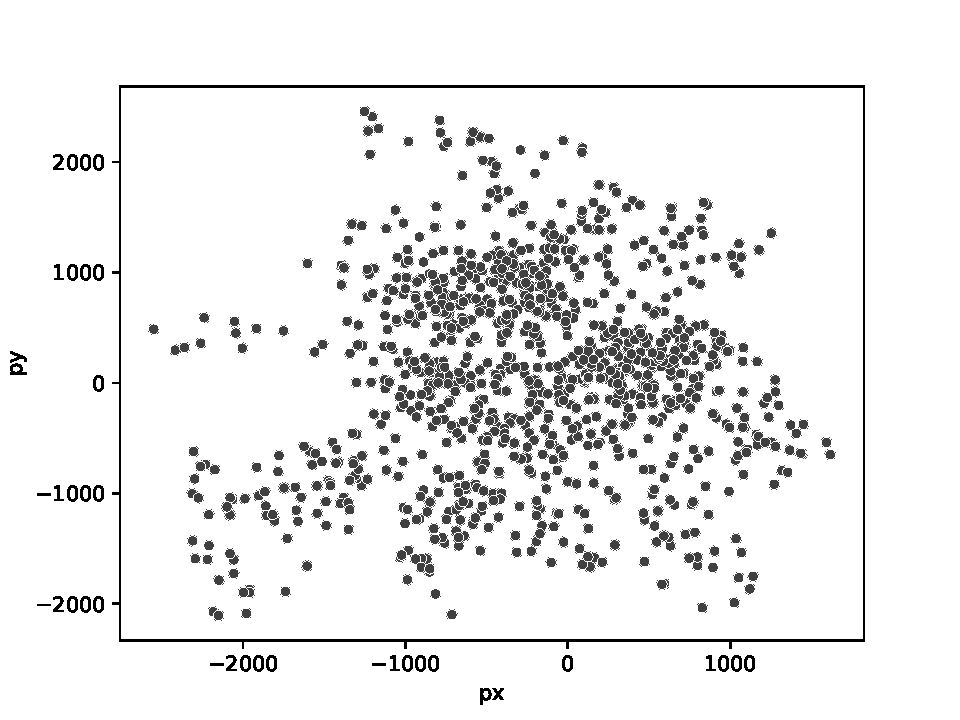
\includegraphics[scale=.41]{scatter_1000_cl0.pdf}
		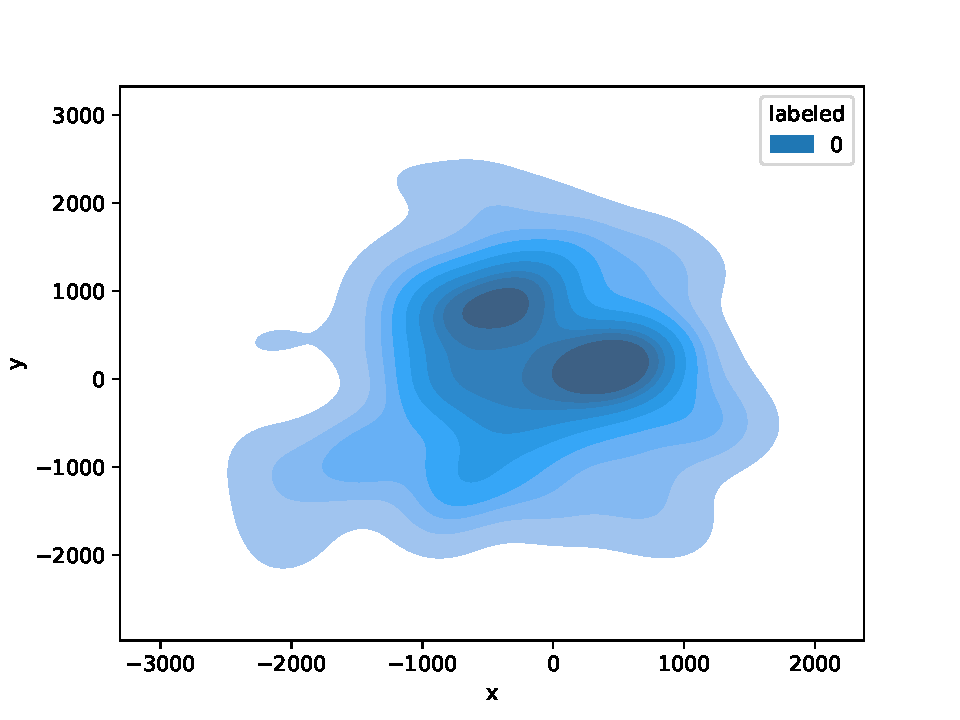
\includegraphics[scale=.41]{density_1000_cl0.pdf}\\
		\centering 100 Größen (100-10000 Pkt.) - 5 Instanzen pro Größe 
		
	
	\end{columns}
	\end{frame}
	
%------------------------------------------------


\begin{frame}
	\frametitle{Phase 2 - Instanzen}
	\textbf{Gleichverteilt}
	\begin{columns}[c] % The "c" option specifies centered vertical alignment while the "t" option is used for top vertical alignment
		
		\column{.9\textwidth} % Left column and width
		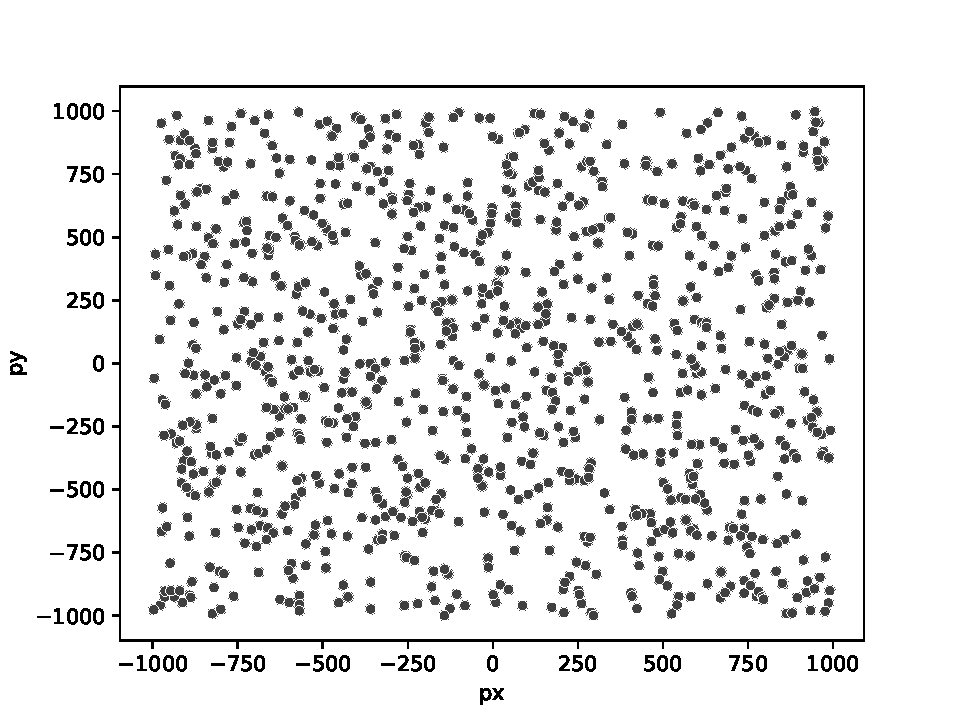
\includegraphics[scale=.41]{scatter_1000_ran0.pdf}
		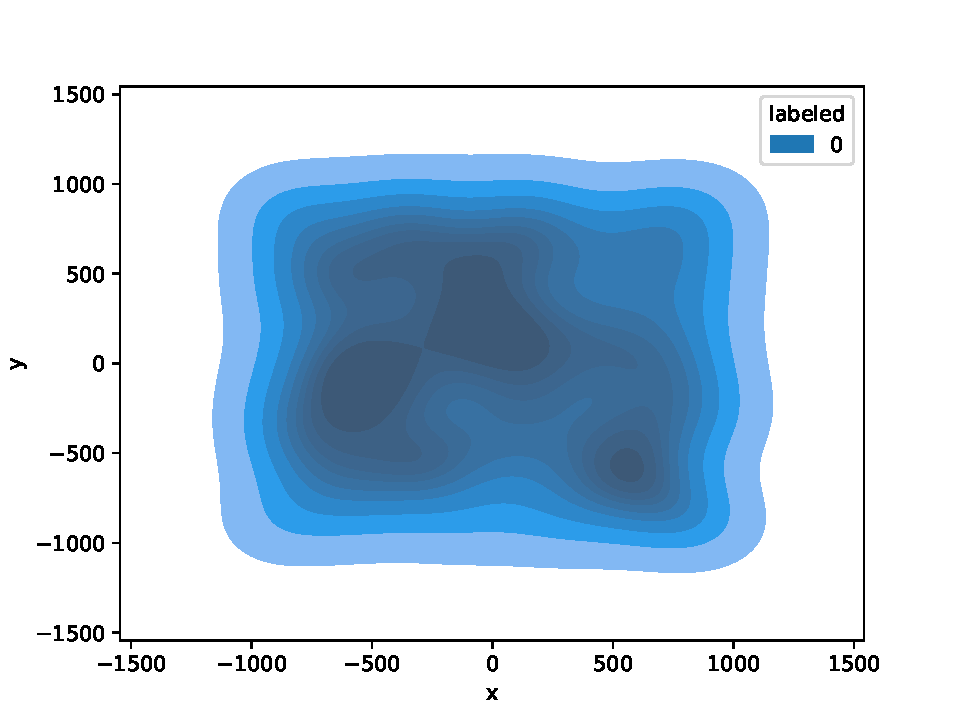
\includegraphics[scale=.41]{density_1000_ran0.pdf}\\
		\centering 100 Größen (100-10000 Pkt.) - 5 Instanzen pro Größe 
		
	
	\end{columns}
	\end{frame}
	
%------------------------------------------------


\begin{frame}
	\frametitle{Phase 2 - Instanzen}
	\textbf{Geographisch}
	\begin{columns}[c] % The "c" option specifies centered vertical alignment while the "t" option is used for top vertical alignment
		
		\column{.9\textwidth} % Left column and width
		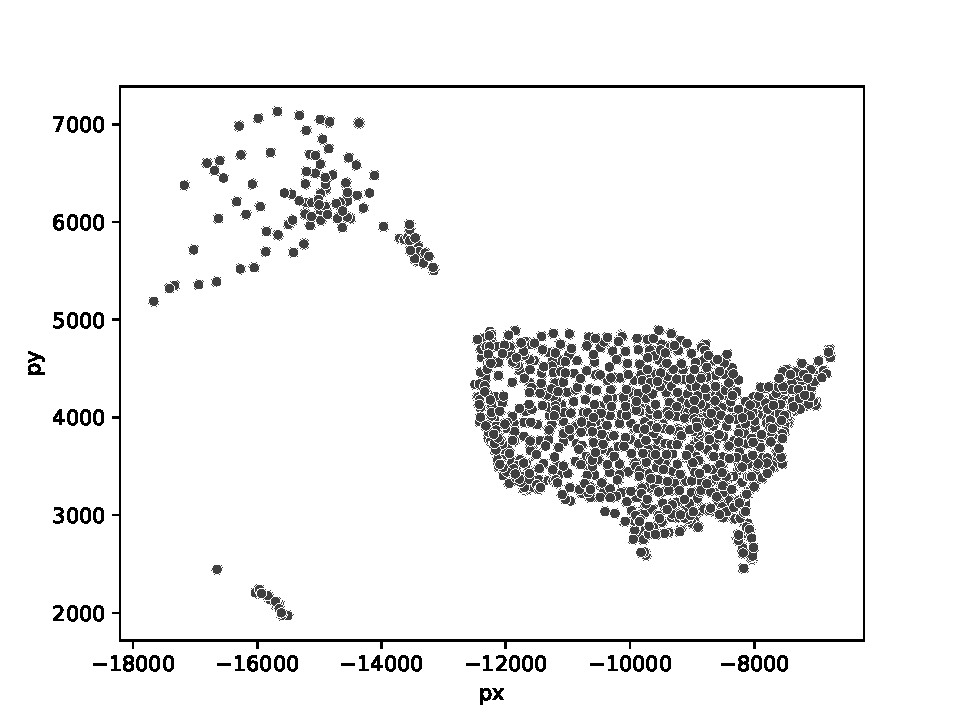
\includegraphics[scale=.41]{scatter_us_cities.pdf}
		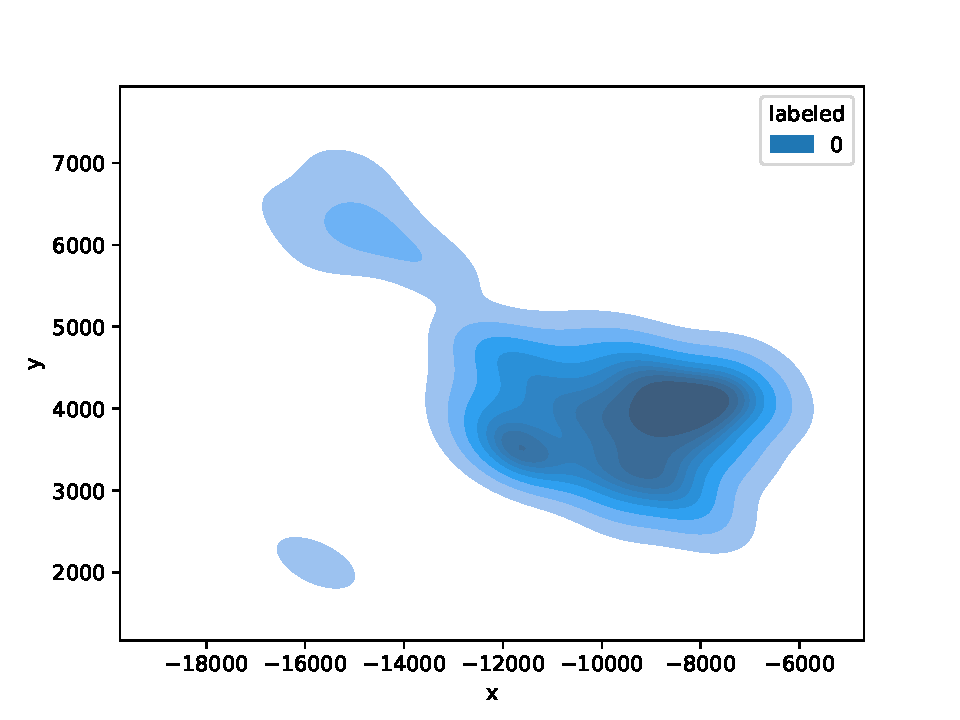
\includegraphics[scale=.41]{density_us_cities.pdf}\\
		\centering 3 Instanzen mit 357 - 1158 Pkt.
		
	
	\end{columns}
	\end{frame}
	
%------------------------------------------------

\begin{frame}
	\frametitle{Phase 2 - Auswertung}
	\textbf{Cluster}
	\begin{columns}[c] % The "c" option specifies centered vertical alignment while the "t" option is used for top vertical alignment
		
		\column{.9\textwidth} % Left column and width
		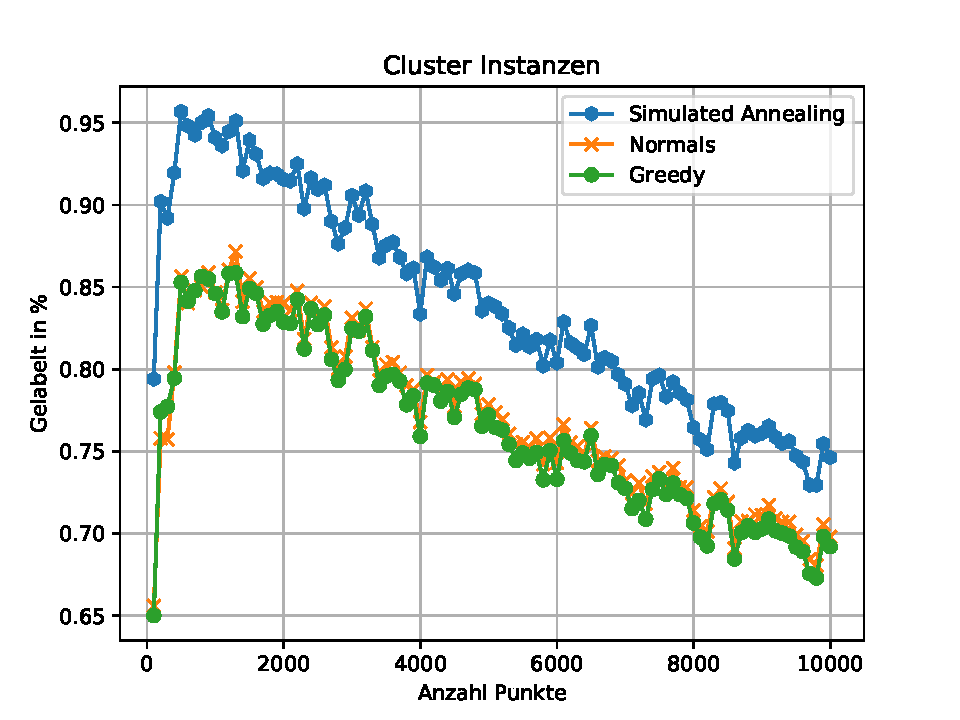
\includegraphics[scale=.41]{cluster_instances.pdf}
		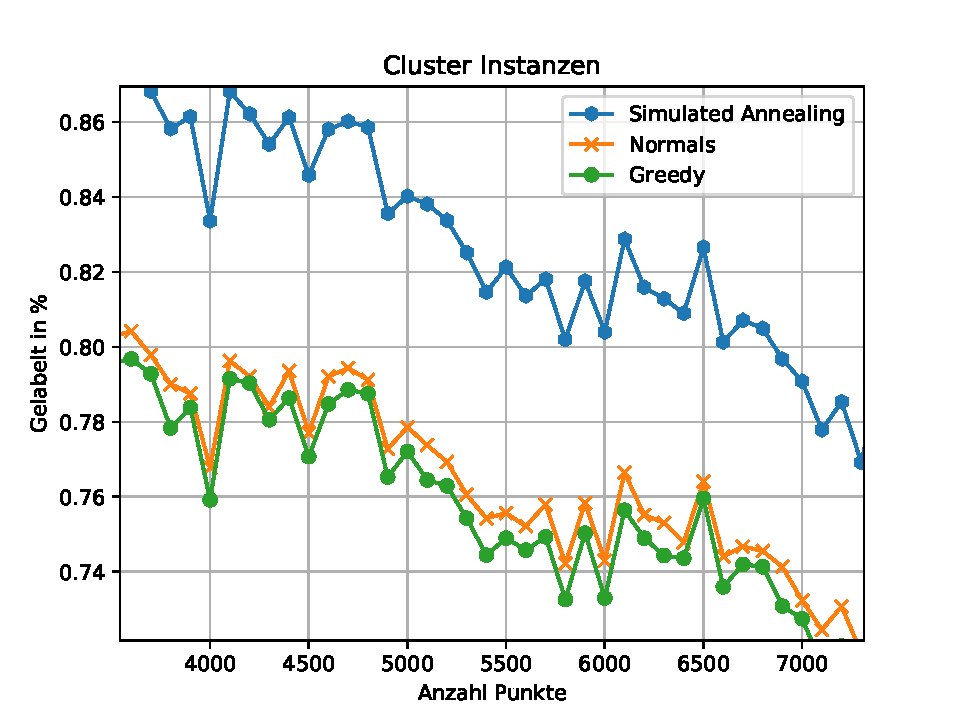
\includegraphics[scale=.41]{cluster_instances_detail.pdf}\\
		
	
	\end{columns}
	\end{frame}
	
%------------------------------------------------


\begin{frame}
	\frametitle{Phase 2 - Auswertung}
	\textbf{Gleichverteilt}
	\begin{columns}[c] % The "c" option specifies centered vertical alignment while the "t" option is used for top vertical alignment
		
		\column{.9\textwidth} % Left column and width
		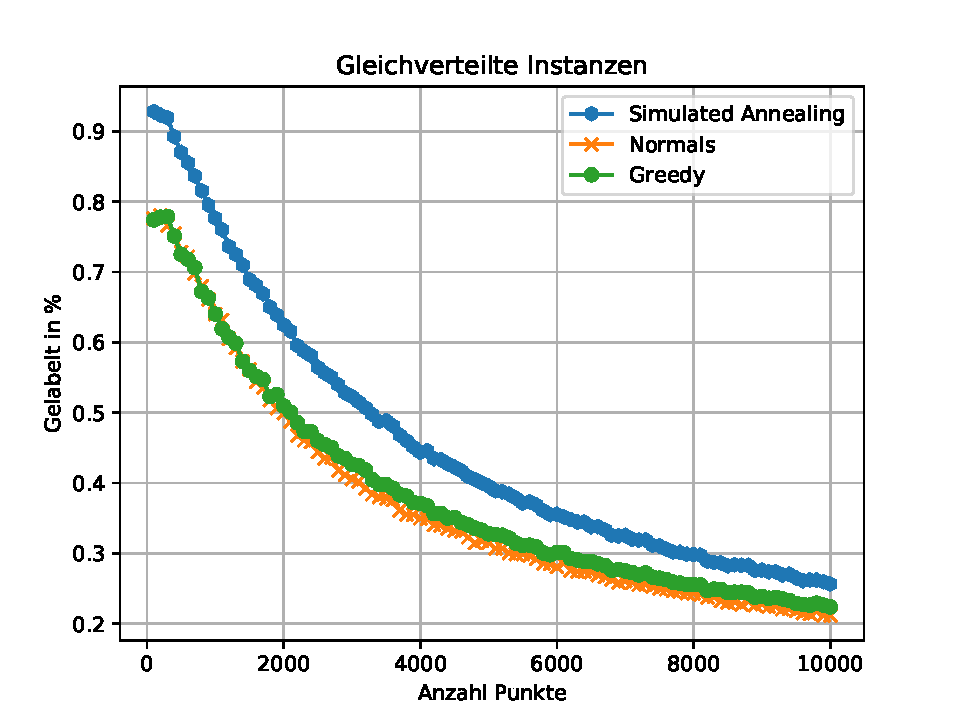
\includegraphics[scale=.41]{random_instances.pdf}
		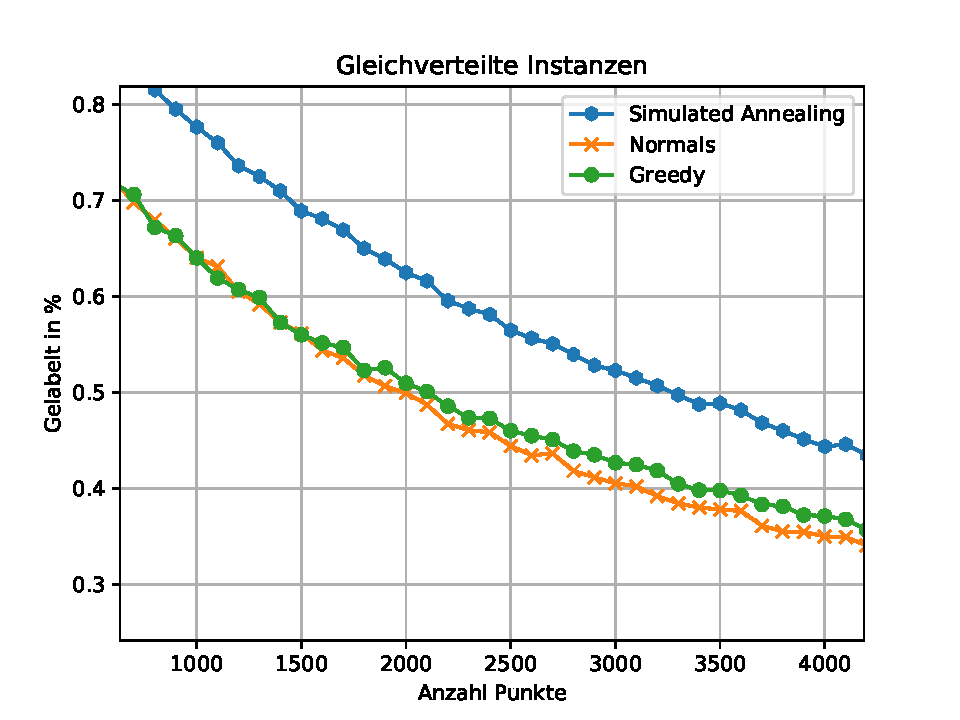
\includegraphics[scale=.41]{random_instances_detail.pdf}\\
		
	
	\end{columns}
	\end{frame}
	
%------------------------------------------------

\begin{frame}
	\frametitle{Phase 2 - Auswertung}
	\textbf{Geographisch}
	\begin{columns}[c] % The "c" option specifies centered vertical alignment while the "t" option is used for top vertical alignment
		
		\column{.9\textwidth} % Left column and width
		\centering 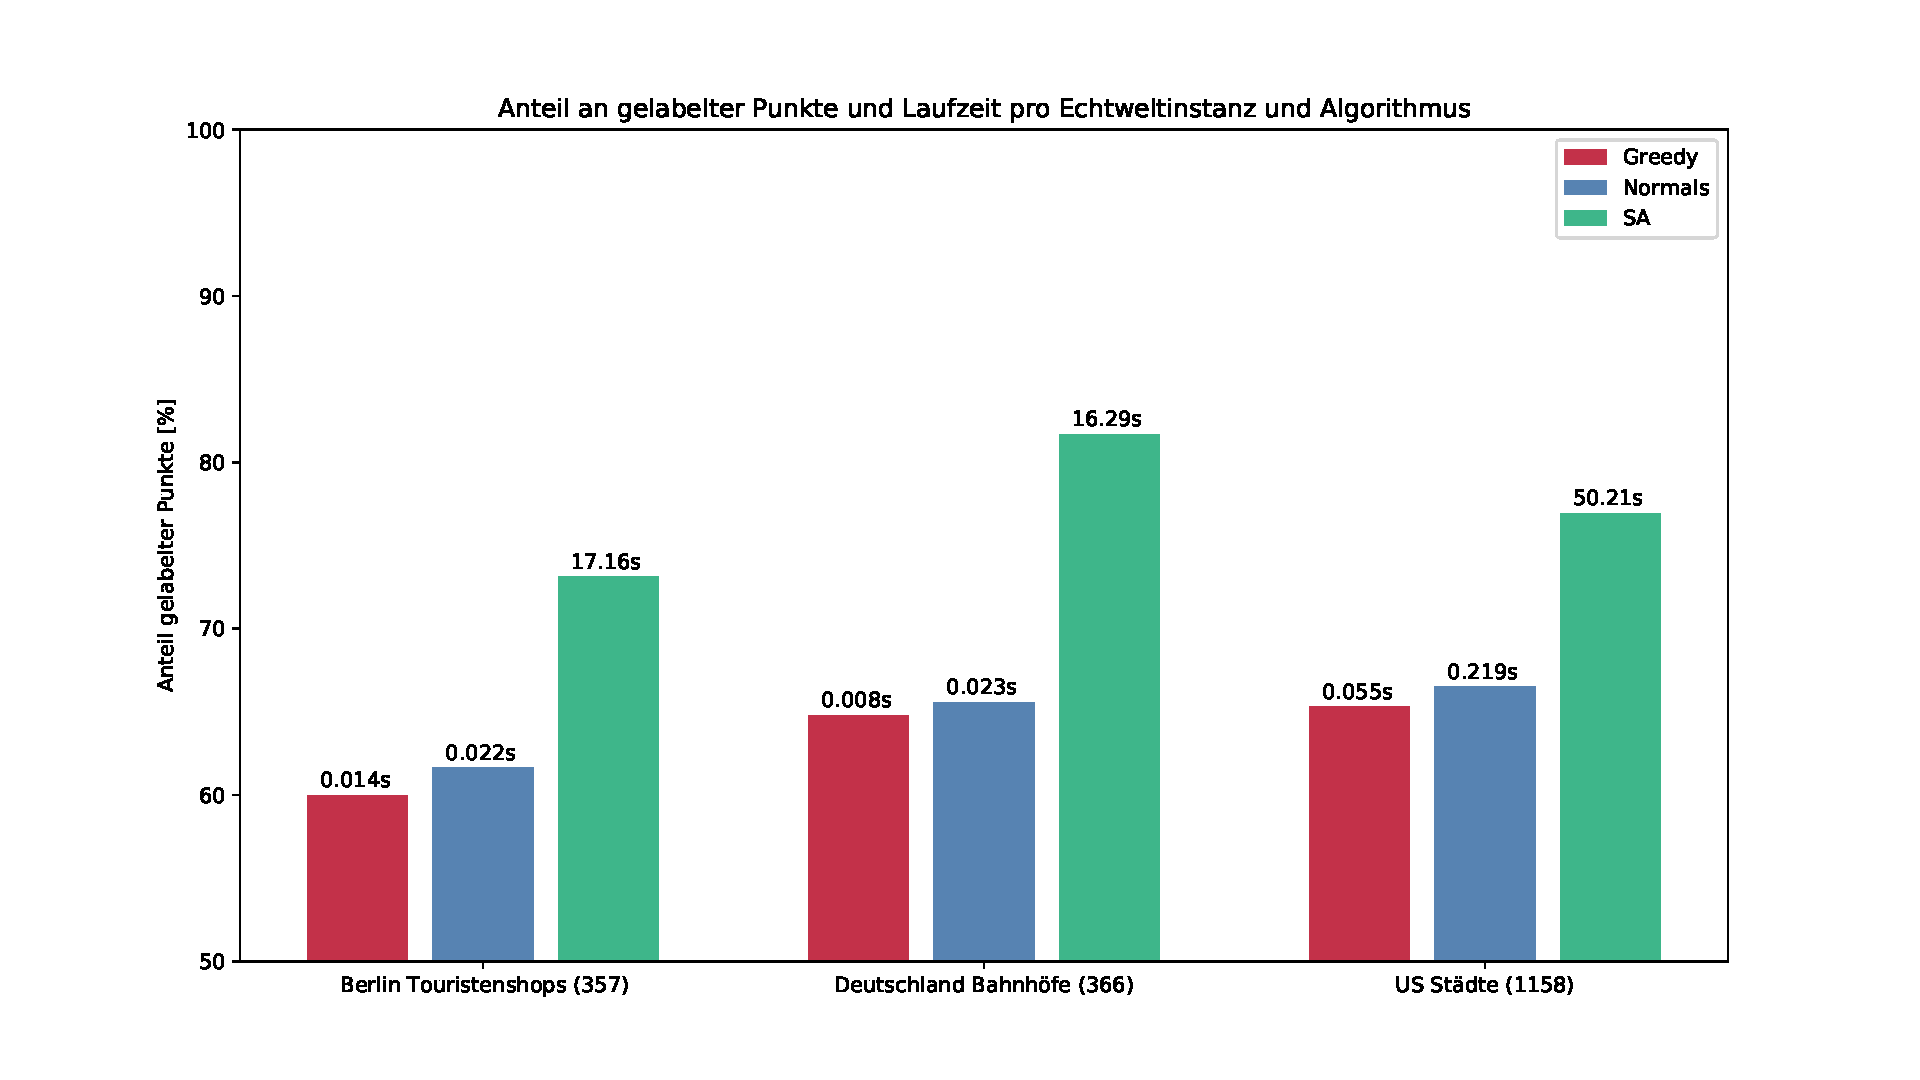
\includegraphics[scale=.38]{barplot.pdf}\\
		
	
	\end{columns}
	\end{frame}
	
%------------------------------------------------

\begin{frame}
	\frametitle{Phase 2 - Parameter}
	
	\begin{columns}[c] % The "c" option specifies centered vertical alignment while the "t" option is used for top vertical alignment
		
		\column{.9\textwidth} % Left column and width
		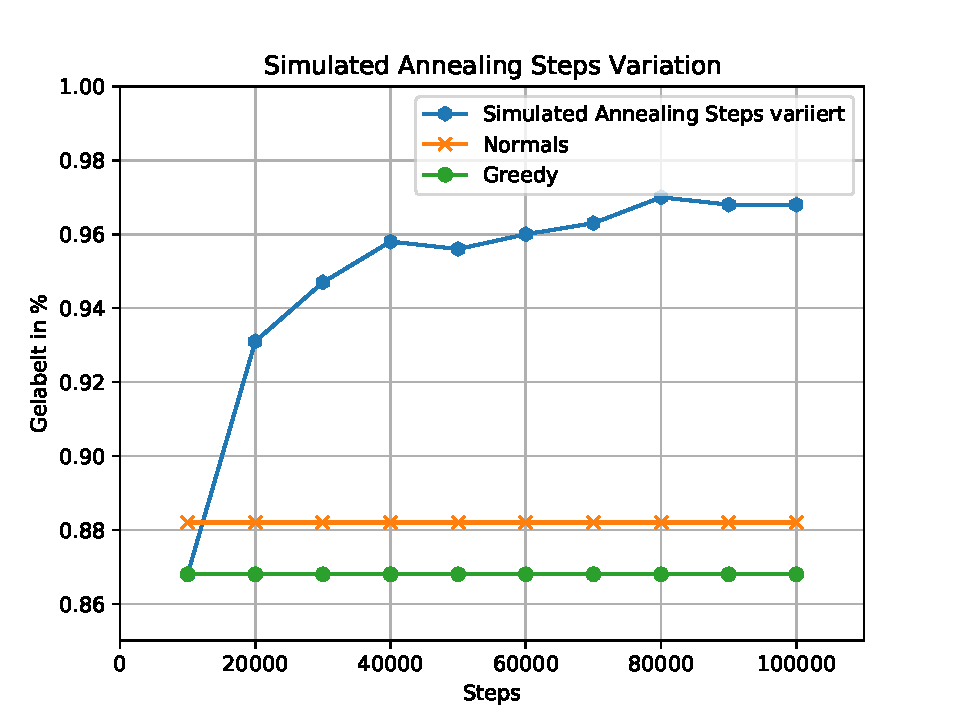
\includegraphics[scale=.41]{sa_variant.pdf}
		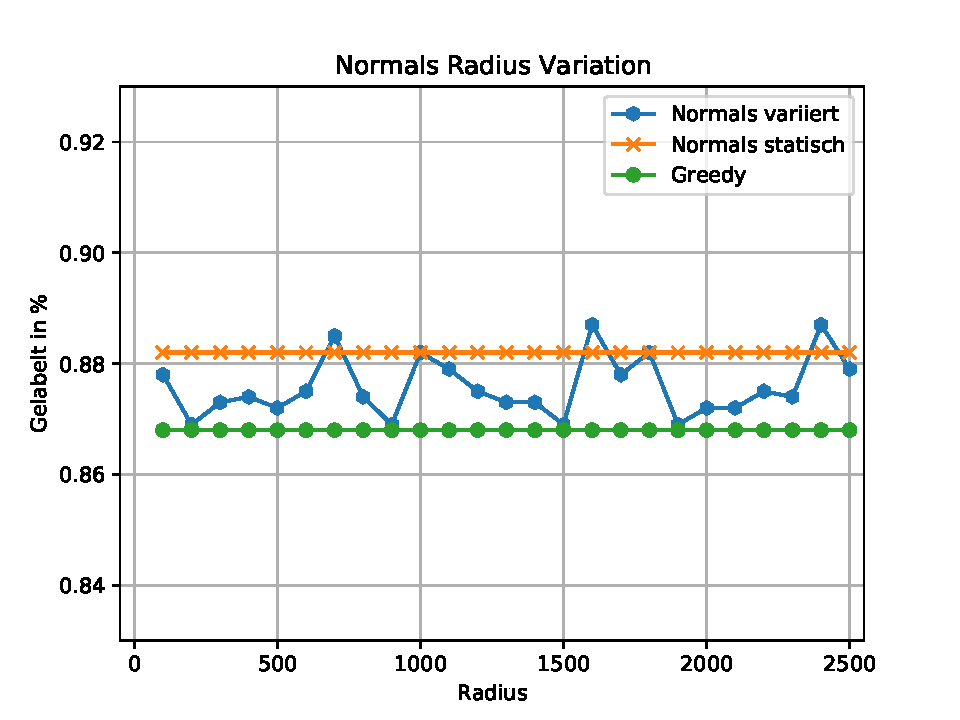
\includegraphics[scale=.41]{normals_variant.pdf}\\
		\centering Variation kritischer Parameter
		
	
	\end{columns}
	\end{frame}
	
%------------------------------------------------



\begin{frame}
	\frametitle{Phase 2 - Ausblick und Verbesserungen}
	\begin{columns}[c] % The "c" option specifies centered vertical alignment while the "t" option is used for top vertical alignment
		
		\column{.30\textwidth} % Left column and width
		\textbf{Allgemein}
		\begin{itemize}
			\item Datenstruktur verbessern
			\item initial mögliche Konflikte berechnen
			\item Symmetrische Distanzmatrix halbieren
			\item []
			
		\end{itemize}
		
		\column{.30\textwidth} % Right column and width
		\textbf{Normals}
		\begin{itemize}
			\item Radius dynamisch bestimmen
			\item andere Nachbarschaftstypen testen
			\item []
			\item []
			
		\end{itemize}
		
	
		\column{.30\textwidth} % Right column and width
		\textbf{Simulated Annealing}
		\begin{itemize}
			\item Abbruchkriterium dynamisch berechnen
			\item Reheating Schedule verbessern
			\item andere Folgen $t_{i}$ testen
			\item verschiedene Nachbarschaften testen
		\end{itemize}\pause
	
	\end{columns}
	\centering \textbf{Fragen?}
	\end{frame}
	
	%------------------------------------------------




\end{document} 